\documentclass[12pt, letterpaper]{article}
\usepackage[utf8]{inputenc}
\usepackage{graphicx}
\usepackage{mathpartir}
\usepackage{textcomp}
\usepackage{gensymb}
\usepackage[tt=false, type1=true]{libertine}
\usepackage[libertine]{newtxmath}
\usepackage[margin=1.0in]{geometry}
\usepackage{hyperref}
\usepackage{pgfplots}
\usepackage[shortlabels]{enumitem}
\usepackage{tikz}
\usepackage{fontawesome}
\usepackage{multicol}
\usepackage{xcolor}
\usetikzlibrary{trees}



\begin{document}
% \tikzstyle{every node}=[draw=black,thick,anchor=west]
% \tikzstyle{a}=[draw=red,fill=red!30]
% \tikzstyle{b}=[draw=blue,fill=blue!30]
% \tikzstyle{c}=[draw=green,fill=green!30]
% \tikzstyle{d}=[draw=orange,fill=orange!30]
% \tikzstyle{e}=[draw=purple,fill=purple!30]
% \tikzstyle{f}=[fill=grey!50]

\newcommand{\FTdir}{}
\def\FTdir(#1,#2,#3){%
  \FTfile(#1,{{\color{black!40!white}\faFolderOpen}\hspace{0.2em}#3})
  (tmp.west)++(0.8em,-0.4em)node(#2){}
  (tmp.west)++(1.5em,0)
  ++(0,-1.3em)
}

\newcommand{\FTfile}{}
\def\FTfile(#1,#2){%
  node(tmp){}
  (#1|-tmp)++(0.6em,0)
  node(tmp)[anchor=west,black]{\tt #2}
  (#1)|-(tmp.west)
  ++(0,-1.2em)
}

\newcommand{\FTroot}{}
\def\FTroot{tmp.west}

\title{
  \textsc{teler}: A Streamlined Version Control System\\
  \large Project Report
}

\author{
  Hadley Luker \and Zachary J. Susag
}

\maketitle
\begin{multicols}{2}
  \section{Project Overview}
  \label{sec:overview}

  During their education, most computer science students must learn to
  use a version control system (VCS). Although these systems see wide
  use in research and industry for software development and
  production, in educational contexts they typically service a
  narrower use case: saving, submitting, and tracking changes in
  programming assignments. This limited use case causes many students
  to become overwhelmed when confronted with the numerous and powerful
  commands available to modern VCSes such as Git and Mercurial. For
  example, the typical workflow of saving changes to a remote
  repository in Git proceeds as follows:

  \begin{enumerate}
  \item \texttt{git add .}
  \item \texttt{git commit -m "Fixed bug."}
  \item \texttt{git push}
  \end{enumerate}

  These three commands are practically an idiom that students are
  habitually trained into, and deviations from this pattern are rare
  and incite confusion. For example, if the \texttt{-m} is omitted
  from the end of \texttt{git commit}, the terminal will run the Vim
  text editor by default in order for the user to write a commit
  message. Due to Vim's unintuitive keybindings and minimal user
  interface, students confronted with this sudden change in
  environment may make errors in the editor or find themselves unable
  to exit and subsequently close the entire hosting terminal window.

  For these reasons, we decided to develop \textsc{teler}: a
  streamlined version control system for the student use case. Our
  system exposes exactly five commands: repository initialization,
  pushing changes with a required commit-like summary to a remote,
  pulling changes from a remote, reverting changes to a specific
  version, and viewing version history. This interface condenses the
  common add-commit-push / pull command sequence at the expense of
  requiring all files to be pushed or pulled at once. However, this
  has positive effects: it encourages users to push frequently and
  document important changes as they are made.

  Our results found that, although Git is a clear winner in terms of
  speed, Teler still performs quickly at directory sizes likely to
  be used by students --- an easy sacrifice to make at such small
  timescales.

  \section{Design \& Implementation}
  \label{sec:desimp}
  The design of our program is centered around two main commands and
  three components: the command line interface, the shadow directory
  which contains all changes recorded by \textsc{teler}, and the
  auxiliary data structures and compression that enable \textsc{teler}
  to be more time and space efficient.

  \subsection{Design}
  \label{subsec:design}
  The use of textsc{teler} depends mostly on two key commands,
  \texttt{push} and \texttt{pull}.

  \subsubsection{\texttt{teler push}}
  \label{subsubsec:push}
  At the heart of any good VCS is the ability to rapidly save
  checkpoints into the repository with a timestamp and a message
  without disrupting the user's workflow. To do this, the VCS must
  find which files have changed, which are new, and which are deleted;
  save these changes into the shadow directory; and bundle these in a
  commit to allow for the commit to be referred to at a later time.

  The \texttt{teler push} algorithm does precisely this. First,
  \texttt{teler push} reads the latest commit from the \texttt{.teler}
  directory and retrieves from the associated commit object the root
  of the object tree. From there, our algorithm recursively traverses
  down this object tree, adding the metadata found within the tree
  objects to a hash table. This hash table will be used to store not only
  the metadata of files from the previous commit, but also any
  new, or changed, files in the pending commit.

  Once the hash table has been fully populated, \texttt{teler push}
  will begin computing which files have been changed by traversing the
  current working directory recursively. Each file within the working
  directory is added to the directory tree by storing the hash of the
  file within it. There are two cases.

  If the file is a regular file, the file is hashed using
  \texttt{openssl}'s implementation of the SHA-1 hashing algorithm.
  The hash is then looked up in the hash table to determine whether
  the file exists already within the shadow directory. If not, the
  file is saved to the appropriate location in the shadow
  directory pointed to by the hash and compressed using the \texttt{zlib}
  compression algorithm. Once saved, the hash, file
  permissions, and human-readable filename (metadata) are placed into the hash
  table. The hash is placed into the directory tree. If the hash was found,
  it's added to the directory tree; there is no need
  to recompress the file, as an identical copy already exists (unless
  there is a hash collision). This is crucial to minimize space
  consumption, as more often than not files do not change with every
  commit. Storing multiple copies of the same file within the
  shadow directory would result in an egregious waste of space.

  If the file is a directory, then a new interior node is made
  within the directory tree and the files are added recursively within the
  directory as children to this new node. Once all children have
  been added, they and their metadatas are hashed to compute the hash of
  the tree. This information is then placed in the hash table.

  Once the directory tree has been constructed, \texttt{teler push}
  will write a commit object containing the hash of the root of the
  directory tree, the previous commit hash (if one exists), the
  author's name and email, a timestamp, and a message provided
  to \texttt{teler push} by a prompt to the user. Once committed, the
  directory tree is traversed, whereby all of the tree objects are
  written to the \texttt{.teler/objects} directory. For each interior
  node of the directory tree, we iterate through each child, look up
  their metadata in the hash table, and write this information to
  the tree object. Once written, the tree file is compressed using
  \texttt{zlib}.

  \begin{center}
    \begin{minipage}{.2\textwidth}
      \begin{tikzpicture}[scale=0.85]%
        \draw[color=black!60!white]
        \FTdir(\FTroot,root,.){ % root: parent = \FTroot
          \FTdir(root,src,\textcolor{red}{src}){ % normal dir: (parentID, currentID, label)
            \FTfile(src,\textcolor{blue}{teler.c}) % file: (parentID, label)
          } \FTdir(root,foo,\textcolor{green}{foo}){
            \FTfile(foo,\textcolor{orange}{bar.c}) }
          \FTfile(root,\textcolor{purple}{README.md})
          \FTdir(root,papers,papers){} };

        % ++(0,-0.5em) % additional space if neded
        % ++(0,-0.5em)
      \end{tikzpicture}
    \end{minipage}
    \begin{minipage}{.25\textwidth}
      \begin{tikzpicture}[scale=0.85]
        \draw[color=black!60!white] \FTdir(\FTroot,root,.teler) {
          \FTdir(root,refs,refs) { \FTdir(refs,heads,heads) {
              \FTfile(heads,master) } } \FTdir(root,objects,objects) {
            \FTdir(objects,2a,2a) {
              \FTfile(2a,\textcolor{red}{fea49eb\ldots}) }
            \FTdir(objects,ed,ed) {
              \FTfile(ed,\textcolor{purple}{b37ac10\ldots}) }
            \FTdir(objects,fa,fa) {
              \FTfile(fa,\textcolor{blue}{7c5bb8a\ldots}) }
            \FTdir(objects,6b,6b) {
              \FTfile(6b,\textcolor{green}{42abcc8\ldots}) }
            \FTdir(objects,ae,ae) {
              \FTfile(ae,\textcolor{orange}{183d7e\ldots}) } }
          \FTfile(root,config) };
      \end{tikzpicture}
    \end{minipage}
  \end{center}

  % \begin{tikzpicture}[%
  %   grow via three points={one child at (0.5,-0.7) and two children
  %   at (0.5,-0.7) and (0.5,-1.4)}, edge from parent
  %   path={(\tikzparentnode.south) |- (\tikzchildnode.west)}]
  %   \node {\texttt{.}} child { node [a]{\texttt{src}} child { node
  %   [b]{\texttt{hello\_world.c}}} } child { node [c]{\texttt{foo}}
  %   child { node [d]{\texttt{bar.txt}}} } child { node
  %   [e]{\texttt{papers}} } child { node [f]{\texttt{README.md}} };
  % \end{tikzpicture}

  \subsubsection{\texttt{teler pull}}
  \label{subsubsec:pull}
  The \texttt{teler pull} algorithm is effectively the inverse of the
  push algorithm; instead of constructing the directory tree
  from the working directory, the tree is constructed from the shadow
  directory. The latest commit object is retrieved in a symmetric
  fashion to \texttt{teler push}. The directory tree is then begun to
  be constructed by adding the root of the object tree as the root of
  the directory tree.

  Each object's hash and metadata inside the tree object is inserted
  into the hash table. If the current object is another tree object, we
  create a new interior node within the directory tree and recursively
  add the node's children by parsing the associated tree object. If
  instead the current object is a blob, nothing special needs to
  be done, and the blob's hash is simply added to the directory tree.

  Before the working directory is populated with the contents of the
  directory tree, it is crucial that the working directory is cleared
  of all residual files. If not done, files from the current state
  will be mixed with those of the latest commit.

  Once the directory tree has been fully built, it is then recursively
  traversed. Each interior node's hash is retrieved, which are
  then used to collect their metadata from the hash table. Using the
  human-readable filename, which is stored in said metadata, a new
  directory with the filename is created. From there, the traversal
  recurses downward and processes each of the interior node's
  children. If one of the children is a blob, the blob is decompressed
  from the shadow directory into a file whose name is the
  human-readable name stored in the hash table.

  \subsection{Implementation}
  \label{sec:implementation}
  \textsc{teler} is a snapshot-driven system, requiring it to save a copy of all
  files when changes are saved. This obviously creates efficiency risks for both
  space and time, as space needed to save these changes and the time needed to
  reload them could both be quite large. Our implementation, focused around the
  ``shadow directory'' in which these changes are stored, attempts to use
  fast and space-efficient methods like hash lookup, compression, and
  uniqueness-based saving in order to meet our efficiency requirements.

  \subsubsection{Shadow Directory}
  \label{subsubsec:shadowdir}
  Within every \textsc{teler} repository is a shadow directory
  appropriately named \texttt{.teler}. The structure of the
  \texttt{.teler} directory is largely influenced by Git.

  Within this directory are two subdirectories:
  \texttt{.teler/refs/heads} and \texttt{.teler/objects}. The
  \texttt{.teler/refs/heads} directory stores a file for each branch
  (currently, only master) which holds the hash of the latest
  commit. This corresponds to a file within the
  \texttt{.teler/objects} directory.

  The \texttt{.teler/objects} directory stores the entire history of
  the repository through snapshots. Directly within this directory are
  numerous subdirectories whose names are two hexadecimal digits.
  Within these subdirectories are files made up of thirty-eight
  hexadecimal digits. Put together, a forty-digit hexadecimal number
  is created which directly corresponds to a uniquely identifying
  SHA-1 hash. These files are what are called objects. Objects are
  broken down into three different types: \textit{trees},
  \textit{blobs}, and \textit{commits}.

  Trees are the mirror of directories in the working directory in that
  they store two different types of objects: trees and blobs. Any
  object within a tree is said to be a \textit{child} of that tree
  object, and \texttt{teler pull} will turn it into a file within the
  directory associated with the tree file. These children
  are referenced by their hash, which is found within a file in the
  \texttt{.teler/objects} directory together with he child's permissions
  and human-readable name. This information is all compressed via
  \texttt{zlib}.

  As trees are to directories, blobs are to regular files. Each blob
  is a compressed version of the contents of a regular file. The name
  of a blob is simply the SHA-1 hash of the contents of the file.
  Blobs are what separates a snapshot-driven implementation of a VCS
  from a delta-driven implementation; instead of storing deltas, or
  changelogs, to reconstruct the files, we instead store the entire
  file (albeit in a compressed form).

  We opted for a snapshot-driven implementation for \texttt{teler} due
  to its slightly better performance in restoring a working directory
  to the state it was at a specified commit (i.e. \texttt{teler
    pull}). A downside is that we consume more space in the process. As
  such, minimizing space consumption was one of the driving goals of
  the design of the shadow directory. We accomplish this through two
  techniques: compression and uniqueness.

  Every file that is stored within the \texttt{.teler/objects}
  directory is compressed using the \texttt{zlib} deflation algorithm,
  aside from those files which are stored within
  \texttt{.teler/refs/heads}. To maintain uniqueness, each blob is
  stored only once within the shadow directory. Since a blob is
  identified by the SHA-1 hash of its contents, we can uniquely identify
  copies of files: they will have the same hash. This property is preserved
  in \texttt{teler push}~(\ref{subsubsec:push}).

  It must be noted that we are relying on not having any
  hash collisions. If a collision happens, either a file would be
  wrongly identified as unchanged and/or portions of a commit would be
  overwritten. However, since SHA-1 can produce $2^{160}$ unique
  hashes, the chance of collisions are miniscule --- especially in an
  environment which is likely to be relatively small, such as a
  repository.

  \subsubsection{Command-Line Interface}
  \label{subsec:cli}

  The command-line interface is a simple argument parser made using
  GNU C's \texttt{argp} interface. This interface automatically
  generates help and syntax information for display on the command
  line through the assignment of certain global variables and ``option
  vectors'', a structure which organizes and configures command line
  arguments. However, our implementation is slightly modified from the
  GNU standard of C argument morphology. The GNU practice is to
  precede all arguments on the command line with a number of hyphens:
  one for single-character arguments (e.g. \texttt{-v}) and two for
  long arguments (e.g. \texttt{--verbose}). We chose to let the first
  argument be hyphen-less. (For differentation's sake, we refer to
  this ``first argument'' as the ``command''.) This reflects more
  closely the practices used by Git for their command line interface,
  which we suspect will be more familiar to students. This decision
  caused us to parse the first argument through an if--else if chain
  and instead use \texttt{argp}'s parser function to parse arguments
  given to the command itself.

  \subsubsection{Data Structures}
  \label{subsec:datastructures}
  In order for \textsc{teler} to be efficient, it must be necessary for
  new or changed files to be rapidly identified; additionally,
  the hierarchical structure of the working directory must be preserved.

  \subsubsection{Hash Table}
  \label{subsubsec:hashtable}

  A dynamic hash table whose keys are SHA-1 hashes and values are
  the associated permissions and human-readable names is used to allow
  for rapid lookup of metadata information. Due to indexing, lookup
  can be done in $\mathcal{O}(1)$ time. Aside from storing the
  metadata information for files, the hash table is crucial for rapidly
  identifying whether a file has been changed.

  As described in section~\ref{subsubsec:push}, before compressing
  blobs into the shadow directory \texttt{teler push} checks to see
  whether an object with an identical hash exists, thus corresponding
  to a file with exactly the same contents. With the hash table, this
  check can be done in $\mathcal{O}(1)$ time; otherwise, we'd have to
  check to see if a file with the hash exists in the
  \texttt{.teler/objects} directory with I/O functions. This would
  incur a significant performance hit.

  \subsubsection{Directory Tree}
  \label{subsubsec:tree}

  The other crucial aspect of \textsc{teler} is preserving
  the hierarchical directory structure of the repository after
  executing \texttt{teler pull}. Since directories are inherently
  trees, we chose to represent both the structure of a commit and the
  working directory as a general tree in which each node has an
  arbitrary number of children. Interior nodes correspond to
  directories, or, equivalently, tree objects, while leaves correspond
  to regular files or blobs. Within each node, the hash of the file is
  stored, which is used to retrieve the metadata information of the
  file from the hash map.

  The directory tree is used in both \texttt{teler
    push}~(\ref{subsubsec:push}) and \texttt{teler
    pull}~(\ref{subsubsec:pull}) for symmetric purposes. During
  pushing, the directory tree is a representation of the working
  directory in memory. During pulling, the directory tree
  represents the object tree of a commit. Thus, the directory tree is
  used to both write the commit to the shadow directory while
  preserving the structure of the directory and to restore the working
  directory from a specified commit. Both of these operations are
  simply recursive tree traversals.

  \subsubsection{Compression}
  \label{subsec:compression}

  As \textsc{teler} saves every version of a file that was added in a
  change, it becomes important to utilize every means of
  space-reduction we have available to us. Therefore, all files and
  commits within a \textsc{teler} repository are compressed. We
  utilize the \texttt{zlib} library to accomplish this. We chose
  \texttt{zlib} because it is free, portable, will essentially never
  expand the data, and has a memory footprint independent of the
  input data. Specifically, we use the deflate algorithm provided by
  \texttt{zlib} in a manner similar to that of \texttt{zpipe}.

  \section{Evaluation}
  \label{sec:evaluation}
  To evaluate \textsc{teler}, we compared its speed in generating
  commits through \textsc{teler push} with Git version 2.17.0. For
  hardware, we used an Intel Core i5-3320M at 3.3GHz with 8GB of RAM
  and a 320GB spinning hard disk. The workstation we used to evaluate
  \textsc{teler} was running Arch Linux with kernal version x86\_64
  Linux 4.16.8-1-ARCH.\@We collected the running times of Git and
  \textsc{teler} using the \texttt{time} command.

  To fairly assess each program we generated a random directory with a
  maximum depth per directory of 3, up to 4 first-level directories,
  and up to 6 maximum children per directory. We then recorded the
  time it took for each program to make a commit of the entire
  directory. This was done ten times, increasing the size of the total
  directory each time. During this process, we also recorded the total
  size of the directory in bytes to be able to compare performance
  based upon size of directory.

  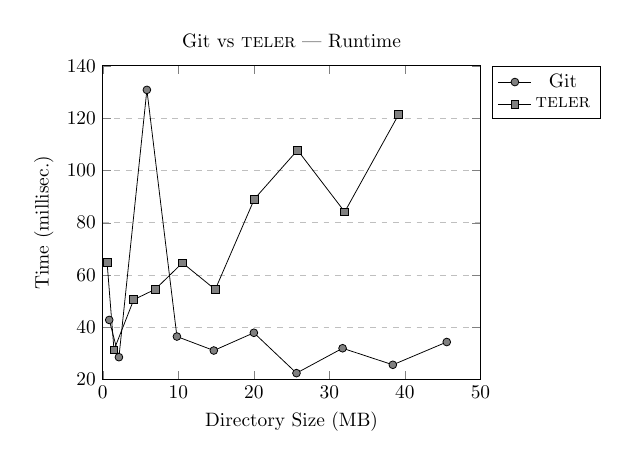
\begin{tikzpicture}[scale=.7]
    \begin{axis}[title={Git vs \textsc{teler} --- Runtime},
      xlabel=Directory Size (MB),ylabel=Time (millisec.),
      ymajorgrids=true, grid style=dashed, xmin=0, xmax=50, ymin=20,
      ymax=140, cycle list name=black white,legend style ={
        at={(1.03,1)}, anchor=north west, draw=black,
        fill=white,align=left}]
      \addplot coordinates
      {(0.863648414611816,42.83645)(2.14697647094727,28.59805)
        (5.84840202331543,130.801418) (9.82489395141602,36.487169)
        (14.7062292098999,31.144624) (20.00954246521,37.923561)
        (25.6488037109375,22.493983) (31.7507152557373,32.009287)
        (38.4010543823242,25.6807) (45.5406074523926,34.394122) };
      \addlegendentry{Git} \addplot coordinates {
        (0.575816154479981,64.931915) (1.4955883026123,31.372593)
        (4.10868740081787,50.585107) (6.95060062408447,54.541024)
        (10.5521659851074,64.661023) (14.8957929611206,54.457689)
        (20.0735664367676,89.068764) (25.7884387969971,107.76408)
        (32.0338525772095,84.147018) (39.1849241256714,121.459343)};
      \addlegendentry{\textsc{teler}}
    \end{axis}
  \end{tikzpicture}

These results demonstrate Git's clear victory in overall speed and fascinating
ability to add and commit in almost constant time relative to the directory
size. However, \textsc{teler} still fulfills its goals of being a simple yet
reasonably efficent VCS; it maintains subsecond times at directory sizes likely
to be found in homework directories for students, even on old hardware, and any
time lag in this case will be perceptually negligible.

\end{multicols}
\end{document}
